% XeLaTeX can use any Mac OS X font. See the setromanfont command below.
% Input to XeLaTeX is full Unicode, so Unicode characters can be typed directly into the source.

% The next lines tell TeXShop to typeset with xelatex, and to open and save the source with Unicode encoding.

%!TEX TS-program = xelatex
%!TEX encoding = UTF-8 Unicode

\documentclass[10pt]{article}
\usepackage{geometry}                % See geometry.pdf to learn the layout options. There are lots.
\geometry{letterpaper}                   % ... or a4paper or a5paper or ... 
%\geometry{landscape}                % Activate for for rotated page geometry
%\usepackage[parfill]{parskip}    % Activate to begin paragraphs with an empty line rather than an indent
\usepackage{graphicx}
\usepackage{amssymb}
%%%% Package
\usepackage{amsmath,amssymb,amsthm}
\usepackage[UTF8,noindent]{ctex}
\usepackage{tikz}
\usetikzlibrary{calc}
\usetikzlibrary{arrows,snakes,backgrounds,shapes,shadows}
\usetikzlibrary{matrix,fit,positioning,decorations.pathmorphing}
\usepackage{listings}
\lstset{
  keywordstyle=\color{blue!70},
  frame=single,
  basicstyle=\ttfamily,
  commentstyle=\small\color{red},
  breakindent=0pt,
  rulesepcolor=\color{red!20!green!20!blue!20},
  rulecolor=\color{black},
  tabsize=4,
  numbersep=5pt,
  breaklines=true,
  %% backgroundcolor=\color{red!10},
  showspaces=false,
  showtabs=false,
  extendedchars=false,
  escapeinside=``,
  frame=no,
}

%%%% New Commands
\newcommand{\blue}{\textcolor{blue}}
\newcommand{\red}{\textcolor{red}}
\newcommand{\purple}{\textcolor{electricpurple}}
\newcommand{\ds}{\displaystyle}
\newcommand{\cd}{\cdots}
\newcommand{\dd}{\ddots}
\newcommand{\vd}{\vdots}
\newcommand{\id}{\iddots}


% Will Robertson's fontspec.sty can be used to simplify font choices.
% To experiment, open /Applications/Font Book to examine the fonts provided on Mac OS X,
% and change "Hoefler Text" to any of these choices.

\usepackage{fontspec,xltxtra,xunicode}
\defaultfontfeatures{Mapping=tex-text}
\setromanfont[Mapping=tex-text]{Hoefler Text}
\setsansfont[Scale=MatchLowercase,Mapping=tex-text]{Gill Sans}
\setmonofont[Scale=MatchLowercase]{Andale Mono}

\begin{document}
\renewcommand{\proofname}{\textbf{证明}}
%%%% New Theorem
\newtheorem{li}{例}
\newtheorem{jielun}{结论}
\newtheorem{dingli}{定理}
\newtheorem{mingti}{{命题}} 
\newtheorem{yinli}{{引理}} 
\newtheorem{tuilun}{{推论}}
\newtheorem{dingyi}{{定义}} 
\newtheorem*{jie}{{解}}
\newtheorem*{zhengming}{{证明}}
\newtheorem{zhu}{{注}}
\newtheorem*{zhu*}{{注}}
\newtheorem{xingzhi}{{性质}}
\newtheorem{wenti}{{问题}}
\newtheorem{xiti}{{习题}}

\title{二叉查找树(Binary Search Tree)}
\author{张晓平}
%\date{}                                           % Activate to display a given date or no date
\maketitle

\section{定义}
\begin{dingyi}
二叉查找树是一棵二叉树,可以是空树,否则满足如下性质:
\begin{enumerate}
\item 树中结点有一个唯一的关键字;
\item 如果有左子树,则左子树的所有关键字小于根的关键字;
\item 如果有右子树,则右子树的所有关键字大于根的关键字;
\item 左、右子树都是二叉查找树。
\end{enumerate}
\end{dingyi}
以上定义是递归的。由性质2、3、4可推出所有关键字都不相同。
\begin{figure}[htbp]
\centering
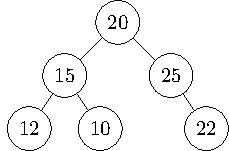
\includegraphics[width=1.5in]{TIKZ/bst/bst1.pdf}  
\caption{不是BST}
\end{figure}
\begin{figure}[htbp]
\centering
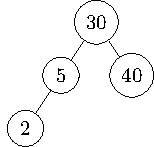
\includegraphics[width=1.in]{TIKZ/bst/bst2.pdf}
\caption{BST}  
\end{figure}
\begin{figure}[htbp]
\centering
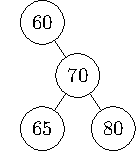
\includegraphics[width=.9in]{TIKZ/bst/bst3.pdf}  
\caption{BST}
\end{figure}
 


\begin{zhu}
二叉查找树特别适合同时需要查找、插入和删除三种操作的应用。二叉查找树可以按关键字值操作,也可以按关键字序操作。如:可在查找树中查找或删除关键字为key的结点,也可以删除关键字排第5小的结点;还可以插入一个结点,同时获得该结点关键字的大小位置。
\end{zhu}

\lstinputlisting[language=C,title=BST结点描述,frame=single]{BST/BSTree.h}

\section{查找}
假设要查找关键字是key的结点。

\subsection{递归实现}
从根开始,若根是NULL,树中无结点,查找失败;否则,比较key与根的关键字:
\begin{itemize}
\item 如果key等于根的关键字,查找成功,结束;
\item 如果key小于根的关键字,因右子树的所有关键字不可能等于key,故应查找根的左子树;
\item 如果key大于根的关键字,应查找根的右子树。
\end{itemize}

\lstinputlisting[language=C,title=BST的查找(递归实现),frame=single]{BST/search.c}

\subsection{非递归实现}
用while结构代替递归结构。
\lstinputlisting[language=C,title=BST的查找(非递归实现),frame=single]{BST/iter_search.c}


\section{插入}
往BST中插入关键字为key的结点,首先应检查该结点是否已经出现在树中,故应先执行查找操作,若查找不成功,则在该位置执行插入操作。

如,在图\ref{insert}中插入80,首先在树中查找80,查找不成功,最后找到结点40,插入80使之成为结点40的右孩子。继续插入35,查找不成功,最后仍找到结点40,插入35使之成为结点40的左孩子。

在整个过程中,若查找不成功,则必须获取最后找到的结点,该功能可以对iter\_search函数略加改动而得到。
\begin{figure}[htbp]
\centering
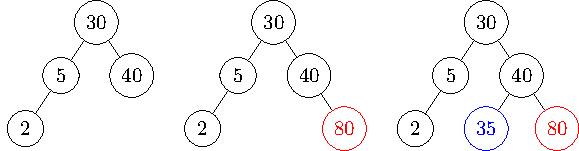
\includegraphics[width=4in]{TIKZ/bst/bst_insert.pdf}  
\caption{插入操作}\label{insert}
\end{figure}


\lstinputlisting[language=C,title=BST的查找(修正),frame=single]{BST/mod_search.c}

\lstinputlisting[language=C,title=BST的插入,frame=single]{BST/insert.c}


\section{删除}
删除操作分为以下三种情形:
\begin{enumerate}
\item 删除叶子结点特别简单。如删除结点35,只需把其父亲的左孩子域置为NULL,然后释放被删除结点的空间即可。
\begin{figure}[htbp]
\centering
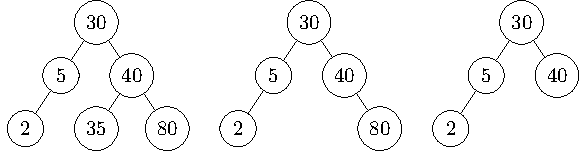
\includegraphics[width=5in]{TIKZ/bst/bst_delete1.pdf}  
\caption{删除叶子结点}\label{delete1}
\end{figure}

例如,在图\ref{delete1}中删除35,只要把其父亲结点40的左孩子域置为NULL,然后释放被删除结点35的空间;接着删除80,将其父亲结点40的右孩子域置为NULL,释放结点80的空间。

\item 若待删结点不是叶子,但只有一个孩子,先把待删结点的空间释放,然后把它唯一的孩子放在删除结点原来的位置即可。

如在图\ref{delete2}中删除结点5,只要把其父亲结点30原本指向结点5的指针改为指向结点2即可。
\begin{figure}[htbp]
\centering
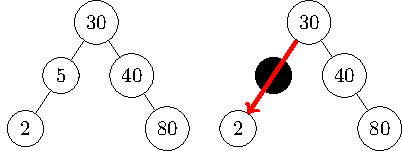
\includegraphics[width=4in]{TIKZ/bst/bst_delete2.pdf}  
\caption{删除只有一个孩子的结点}\label{delete2}
\end{figure}
\item 若待删结点有两个孩子,先用左子树中关键字最大的孩子的data或右子树中关键字最小的孩子的data替换待删结点的data,然后删除子树中的那个结点。

例如,要删除图\ref{delete3}中的结点30,一种做法是用左子树中最大关键字为5的结点替换,另一种做法是用右子树中最小关键字为40的结点替换。以第一种做法为例,将结点5的data存入根结点,然后删除根左边关键字为5的结点,最后将根的左孩子域指向结点2。
\begin{figure}[htbp]
\centering
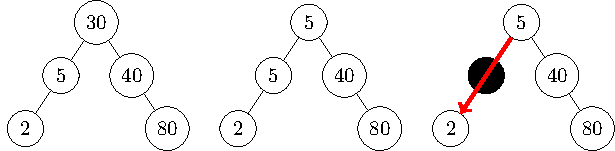
\includegraphics[width=5in]{TIKZ/bst/bst_delete3.pdf}  
\caption{删除有两个孩子的结点}\label{delete3}
\end{figure}
\end{enumerate}

\begin{xiti}
编制程序,实现BST的删除操作。
\end{xiti}

\end{document}  